\chapter{Handshaking}

\section{Handshaking}

Progettare, implementare in VHDL e testare mediante simulazione un sistema composto da 2 nodi, A e B, che comunicano mediante un protocollo di handshaking. Il nodo A e il nodo B possiedono entrambi una memoria interna in cui sono memorizzate N stringhe di M bit, denominate X(i) e Y(i) rispettivamente (i=0,…,N-1). Il nodo A trasmette a B ciascuna stringa X(i) utilizzando un protocollo di handshaking; B, ricevuta la stringa X(i), calcola S(i)=X(i)+Y(i) e immagazzina la somma in opportune locazioni della propria memoria interna.
Per il progetto è possibile considerare una implementazione di tipo comportamentale per effettuare la somma, mentre è necessario prevedere esplicitamente un componente contatore sia nel sistema A sia nel sistema B per scandire la trasmissione/ricezione delle stringhe e per terminare la comunicazione.

\subsection{Architettura}

La soluzione è stata realizzata con un approccio strutturale, partendo dalla creazione dei due sistemi separati, A e B, e procedendo con l'interconnessione di essi. 

In particolare, il sistema A è composto da:
\begin{itemize}
    \item \textit{contatore}: conta il numero di trasmissioni dei dati, in modo tale da terminare opportunamente lo scambio di messaggi;
    \item \textit{rom}: dove sono contenuti i valori delle stringhe da inviare;
    \item \textit{rete di controllo}: regola che la trasmissione dei dati avvenga in modo corretto.
\end{itemize}

Il sistema B, invece, è composto da:
\begin{itemize}
    \item \textit{contatore}: conta il numero di ricezioni dei dati, in modo tale da terminare opportunamente lo scambio di messaggi;
    \item \textit{rom}: dove sono contenuti i valori delle stringhe da sommare;
    \item \textit{registro}: memorizza la stringa ricevuta da A;
    \item \textit{rete di controllo}: regola che la ricezione dei dati e la somma delle stringhe avvenga in modo corretto.
    \item \textit{memoria interna}: dove viene memorizzato il valore ottenuto dalla somma.
\end{itemize}

L'interconnessione tra i due sistemi è visibile nella seguente architettura: 
\begin{figure}[H]
    \centering
    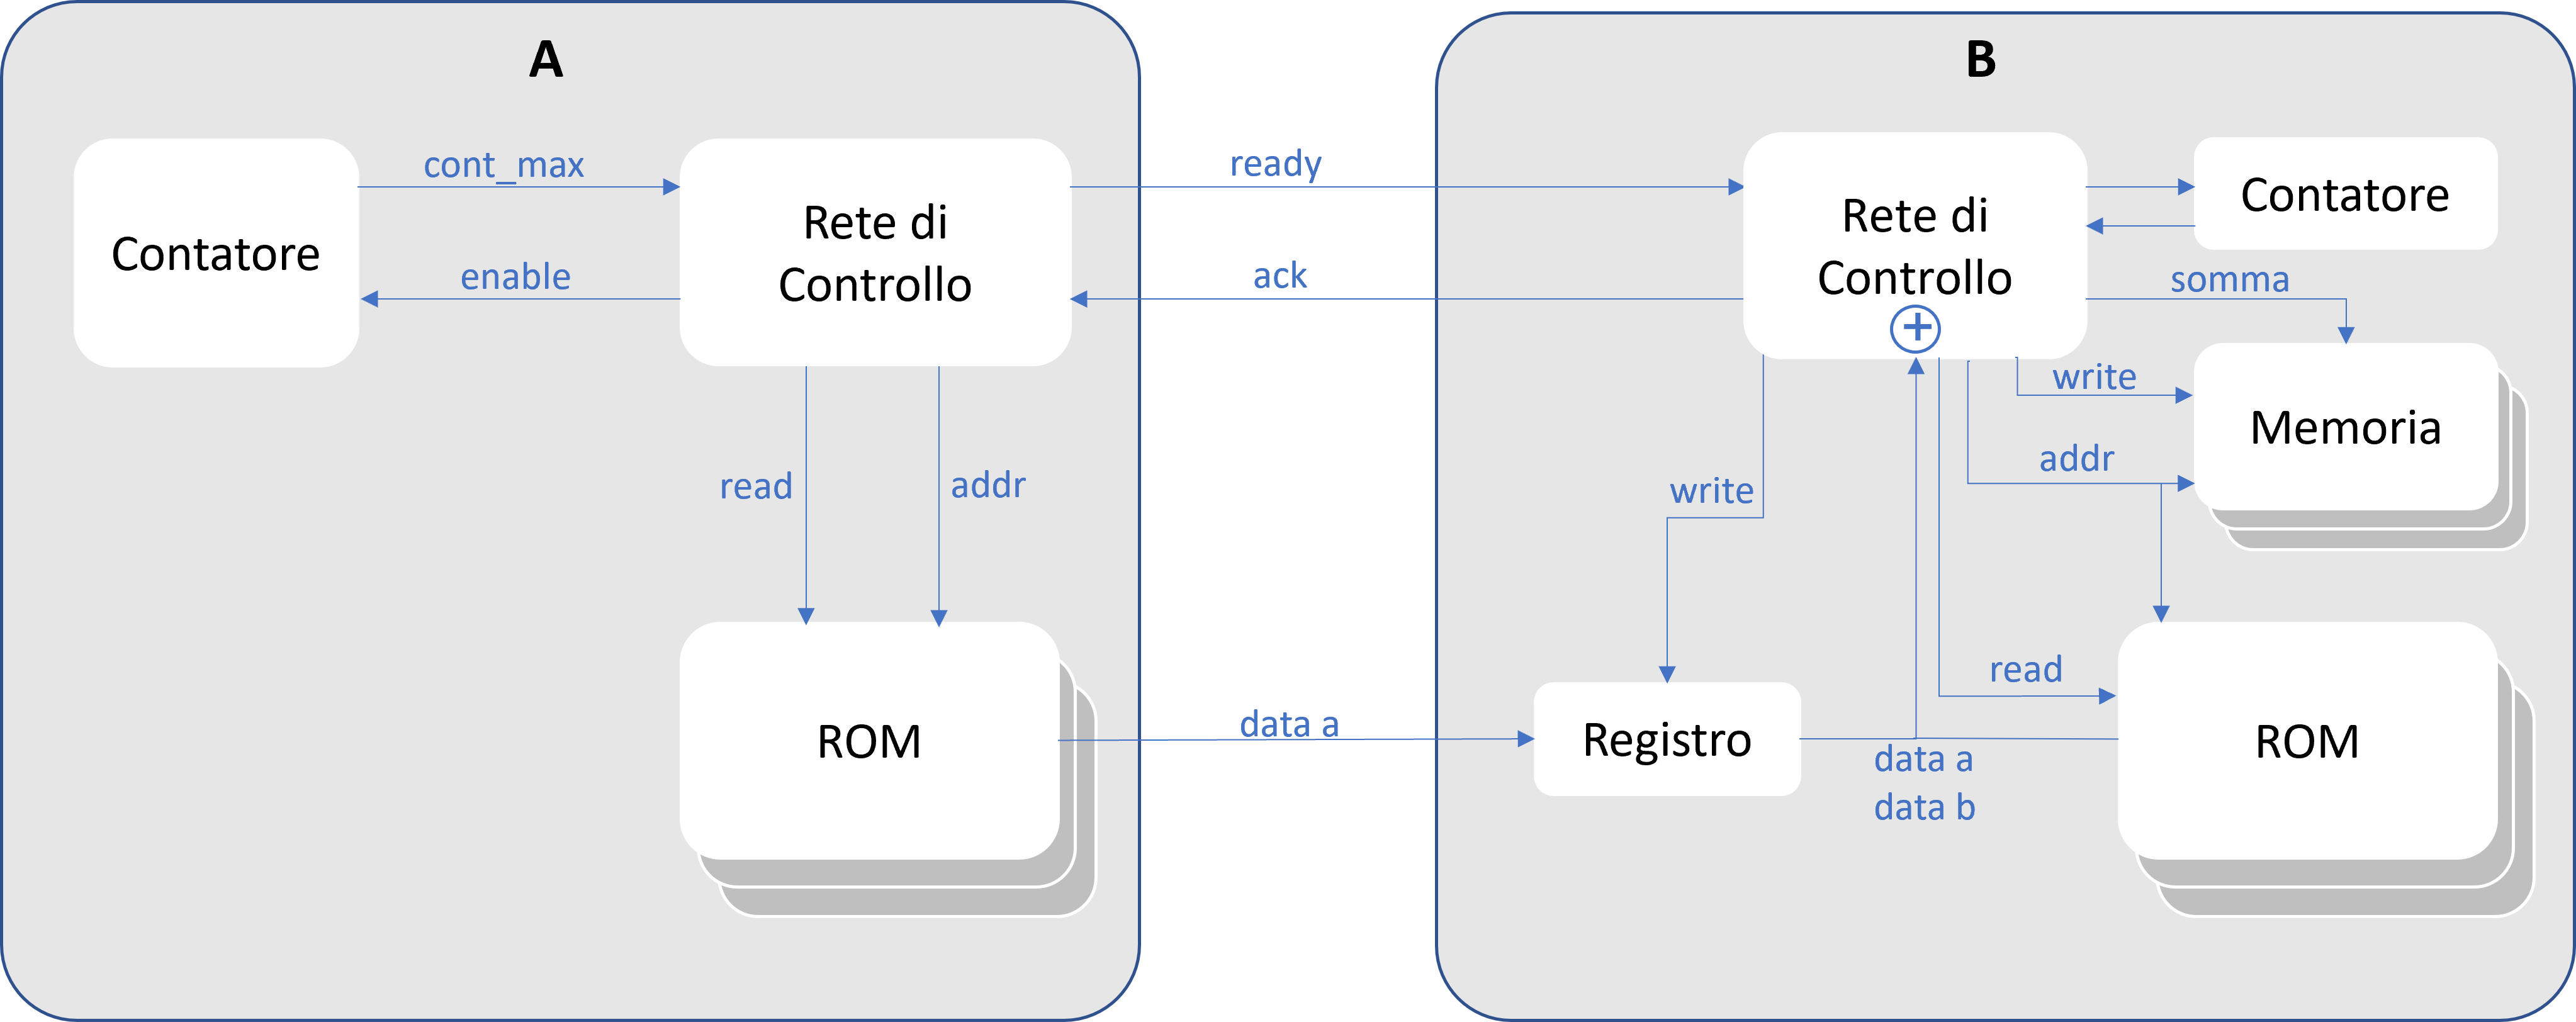
\includegraphics[width=16cm]{immagini/esercizio7/schema_7.1.png}
    \caption{Schema Handshaking}
    \label{fig:my_label}
\end{figure}

Di seguito è possibile osservare la stesura degli automi dei singoli sistemi: 
\begin{figure}[H]
    \centering
    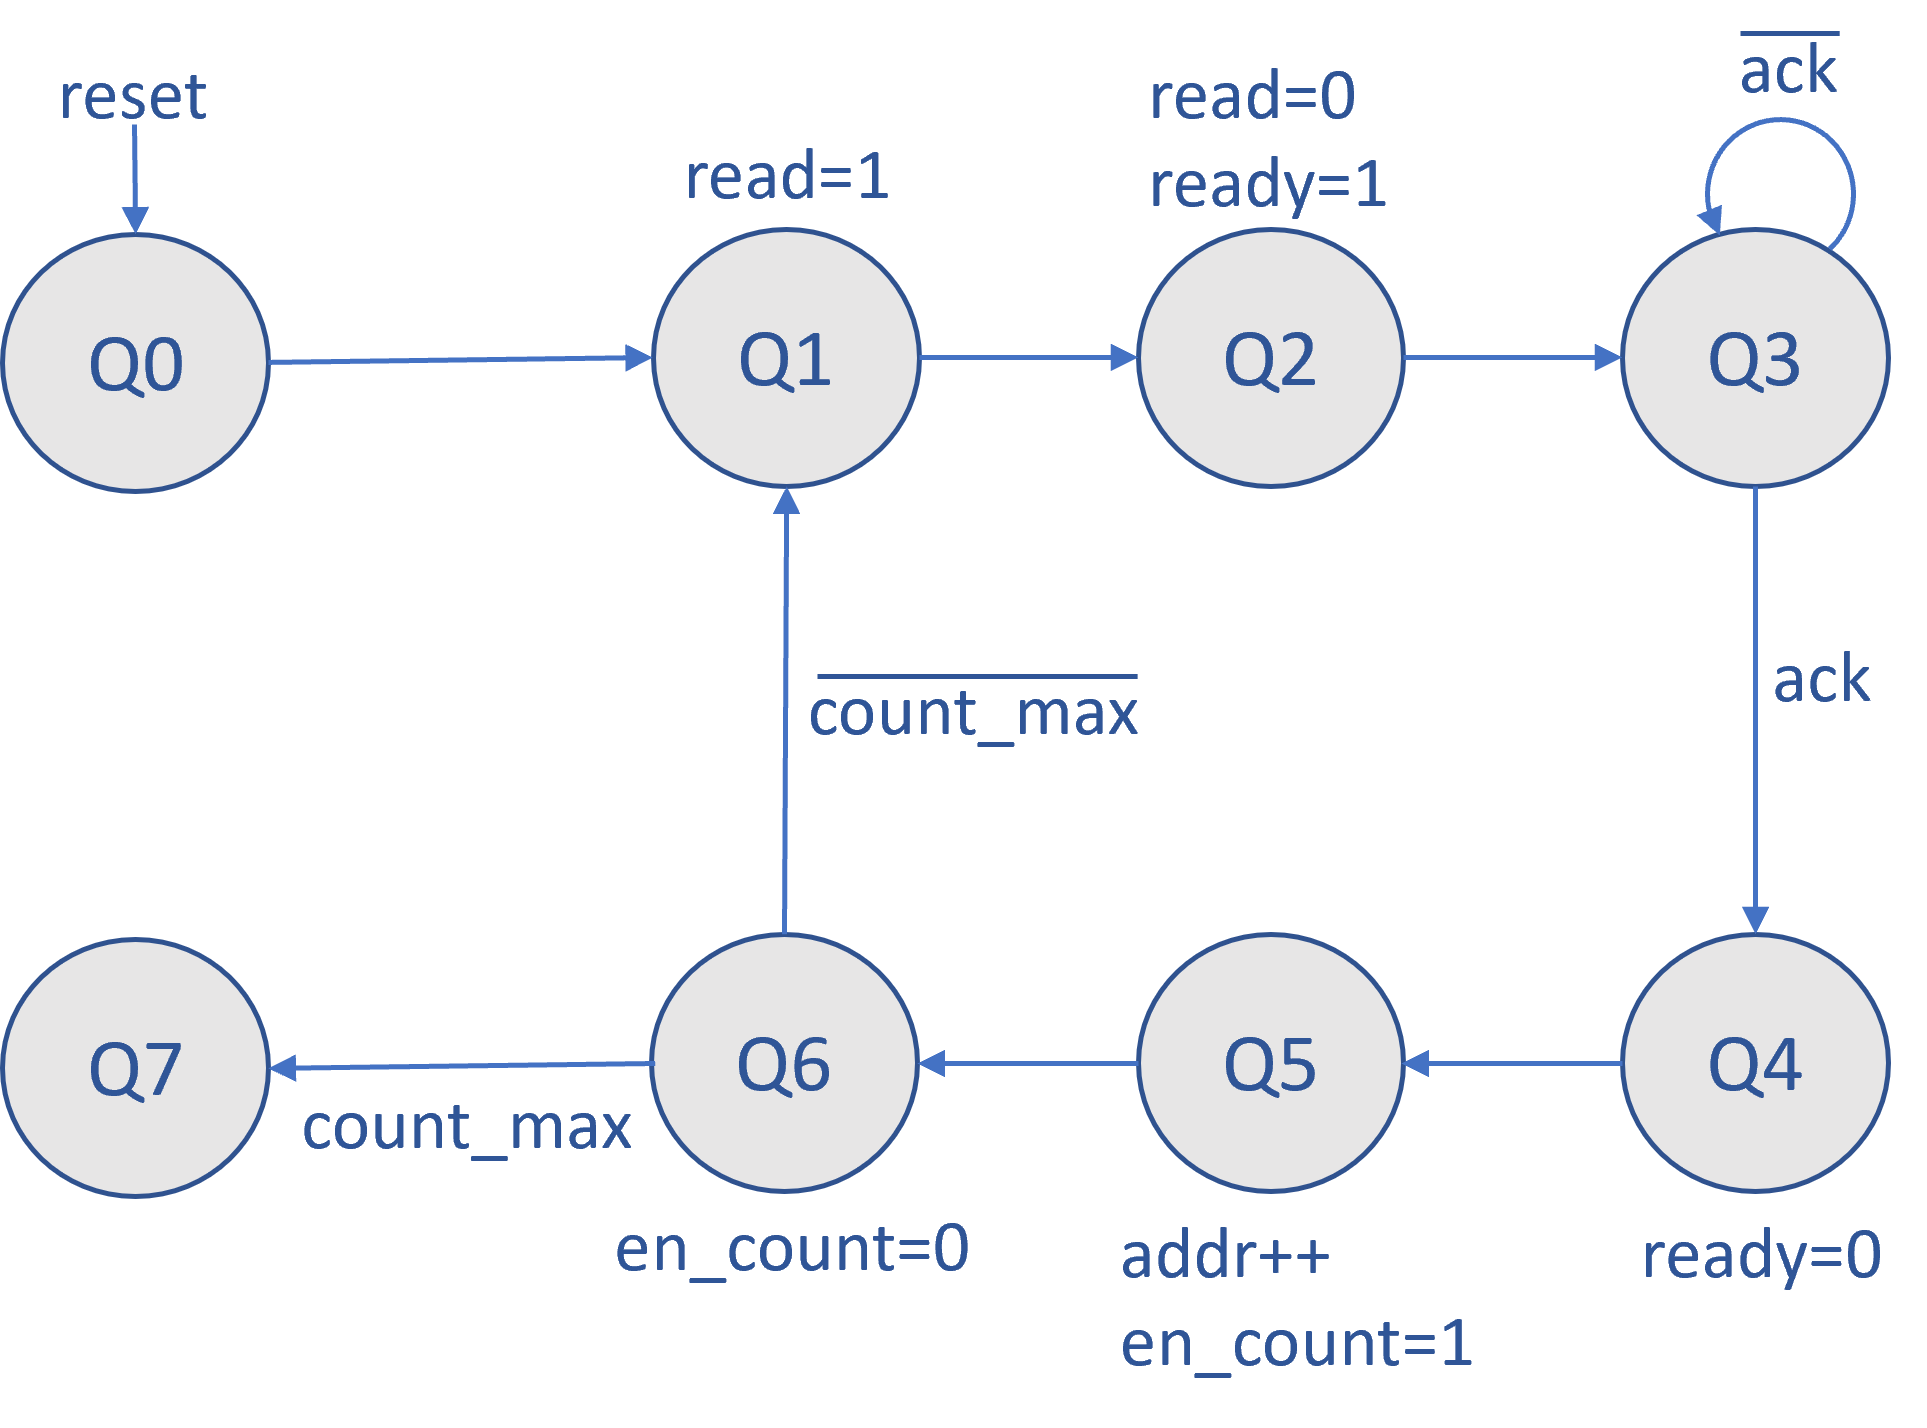
\includegraphics[width=12cm]{immagini/esercizio7/automa_a.png}
    \caption{Automa A}
    \label{fig:7_automa_a}
\end{figure}

\begin{figure}[H]
    \centering
    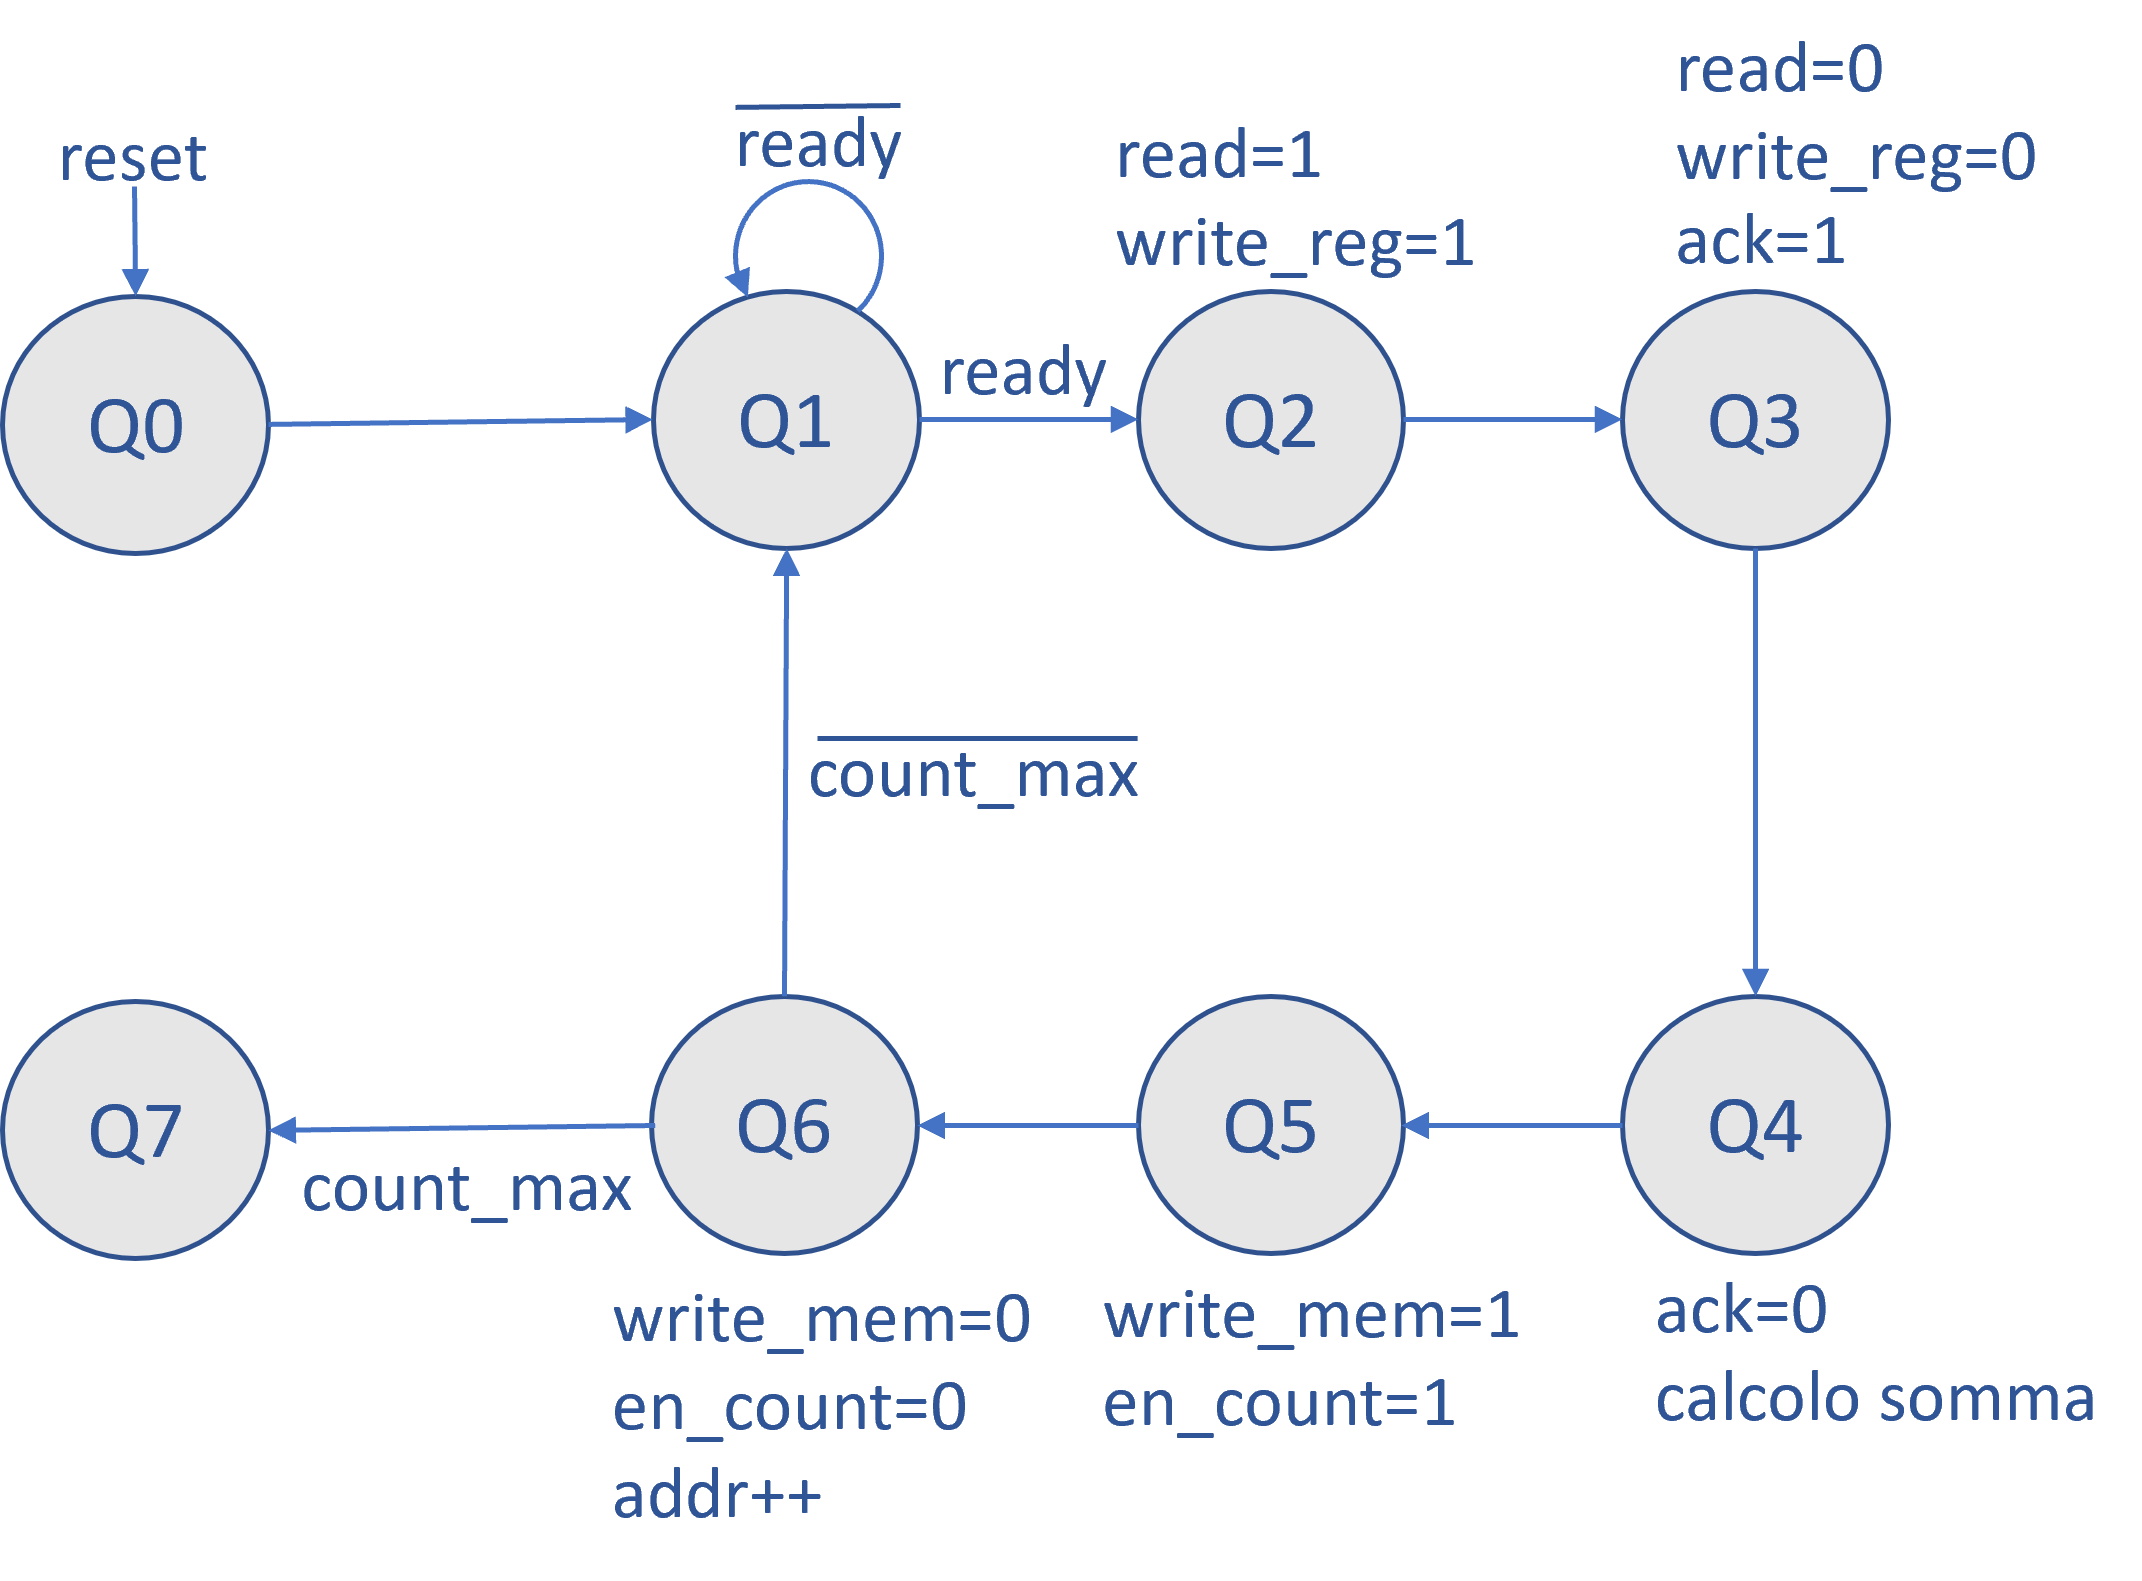
\includegraphics[width=12cm]{immagini/esercizio7/automa_b.png}
    \caption{Automa B}
    \label{fig:7_automa_b}
\end{figure}
Gli stati di particolare interesse sono Q3 per A e Q1 per B. In questi stati infatti si aspetta il segnale generato dall'altro interlocutore, in modo da sincronizzare la comunicazione. Q1 aspetta che il segnale ready sia alzato da A, che indica la possibile trasmissione del dato, Q3 aspetta l'ack che viene alzato da B , che indica l'avvenuta ricezione e scrittura in memoria del dato. I dati vengono memorizzati in un registro temporaneo prima di essere inviati alla rete di controllo per la somma, in modo da poter controllare il momento in cui vengono acquisiti e garantire che non cambino nel tempo.  
Il contatore tiene traccia di quante trasmissioni sono avvenute, e arrivato al massimo invia un segnale \textit{count\_max} che porterà gli automi negli stati Q7, ovvero in idle. 

Sarà necessario un reset per poter ricominciare la trasmissione da capo. 
Un altro aspetto importante riguarda la tempistica con cui si incrementa l'indirizzo addr, necessario a leggere e scrivere nelle memorie dei componenti. Bisogna assicurarsi di completare la scrittura prima dell'incremento, o si rischia di saltare la prima cella di memoria. 
La somma viene effettuata direttamente all'interno del processo della rete di controllo  di B. Tutti gli altri componenti sono stati realizzati a partire da quelli esaminati nei capitoli precedenti, dove è possibile trovarne una descrizione dettagliata.

Di seguito è mostrato il codice dei componenti di A:
\begin{lstlisting} [language=VHDL, caption= Contatore A]
library IEEE;
use IEEE.STD_LOGIC_1164.ALL;
use IEEE.NUMERIC_STD.ALL;

entity contatore is
    Port ( clock : in  STD_LOGIC;
         reset : in  STD_LOGIC;
         enable : in STD_LOGIC;
         counter : out  STD_LOGIC_VECTOR (1 downto 0);
         tc: out std_logic
        );
end contatore;

architecture Behavioral of contatore is

    signal c : std_logic_vector (1 downto 0) := (others => '0');

begin
    counter <= c;
    counter_process: process(clock)
    begin
        if (clock'event AND clock = '1') then
            if (reset = '1') then
                c <= (others => '0');
            else
                if (c="11") then
                    tc<='1';
                elsif (enable='1') then
                    tc<='0';
                    c <= std_logic_vector(unsigned(c) + 1);
                end if;
            end if;
        end if;
    end process;
end Behavioral;


\end{lstlisting}

\begin{lstlisting} [language=VHDL, caption=Rom A]
library ieee;
use ieee.std_logic_1164.all;
use ieee.std_logic_unsigned.all;

entity rom_a is
port(
    clk, read : in std_logic; 
    addr : in std_logic_vector(1 downto 0);
    data : out std_logic_vector(3 downto 0)
    );
end rom_a;

architecture behavioral of rom_a is 
type rom_type is array (0 to 3) of std_logic_vector(3 downto 0);
signal ROM : rom_type := (
    "0010", 
    "0110", 
    "1001", 
    "1111"
);

begin
process(clk)
  begin
    if rising_edge(clk) then
        if read = '1' then
            data <= ROM(conv_integer(addr));
        end if;
    end if;
end process;
end behavioral;
\end{lstlisting}

\begin{lstlisting} [language=VHDL, caption=Rete di controllo A]
library IEEE;
use IEEE.STD_LOGIC_1164.ALL;
use ieee.numeric_std.all;

entity rc_a is
    Port(
        clk,reset,ack: in std_logic;
        count_max :in std_logic;
        en_count,read,ready: out std_logic;
        addr: out std_logic_vector(1 downto 0)
    );
end rc_a;

architecture behavioral of rc_a is

    type stato is (Q0, Q1, Q2, Q3, Q4, Q5, Q6, Q7);
    signal stato_corrente : stato:= Q0;
    signal stato_prossimo : stato;
    signal s_addr: std_logic_vector(1 downto 0) :=(others => '0');

begin
    comb: process(stato_corrente, ack)
       
    begin
        case stato_corrente is
            
            when Q0=>
                stato_prossimo<=Q1;
                s_addr <= "00";
                read<='0';
                ready<='0';
                en_count<='0';

            when Q1=>
                read<='1';
                stato_prossimo<=Q2;

            when Q2=>
                read<='0';
                ready<='1';
                stato_prossimo<=Q3;

            when Q3=>
                if(ack='1') then
                    stato_prossimo<=Q4;
                else
                    stato_prossimo<=Q3;
                end if;

            when Q4=>
                ready<='0';
                stato_prossimo <=Q5;

            when Q5=>
                s_addr <= std_logic_vector( unsigned(s_addr) + 1);
                en_count <='1';
                stato_prossimo <=Q6;

            when Q6=>
                en_count <='0';
                if (count_max ='1') then
                    stato_prossimo <=Q7;
                else
                    stato_prossimo <=Q1;
                end if;

            when Q7=>
                stato_prossimo <=Q7;

            when others => stato_prossimo<= Q0;
        end case;
    end process comb;
 addr <= s_addr;

    seq: process(clk)
    begin
        if rising_edge(clk) then
            if(reset='1')then
                stato_corrente<=Q0;
            else
                stato_corrente<=stato_prossimo;
            end if;
        end if;
    end process seq;
end behavioral;
\end{lstlisting}

Il sistema A, di tipo "Structural", è stato implementato nel seguente modo:
\begin{lstlisting} [language=VHDL, caption= A]
library IEEE;
use IEEE.STD_LOGIC_1164.ALL;

entity A is
    Port (
        clock, ack, reset: in std_logic ;
        ready: out std_logic;
        data: out std_logic_vector (3 downto 0)
    );
end A;

architecture Structural of A is
    component  contatore is
        Port (
            clock : in  STD_LOGIC;
            reset : in  STD_LOGIC;
            enable : in STD_LOGIC;
            counter : out  STD_LOGIC_VECTOR (1 downto 0);
            tc: out std_logic
        );
    end component contatore;

    component rc_a is
        port(
            clk,reset,ack: in std_logic;
            count_max :in std_logic;
            en_count,read,ready: out std_logic;
            addr: out std_logic_vector(1 downto 0)
        );
    end component  rc_a;

    component rom_a is
        port(
            clk, read : in std_logic;
            addr : in std_logic_vector(1 downto 0);
            data : out std_logic_vector(3 downto 0)
        );
    end component  rom_a;

    signal s_count_max:std_logic_vector(1 downto 0):="11";
    signal s_addr:std_logic_vector(1 downto 0):="00";
    signal s_tc, s_en_count, s_read:std_logic :='0';

begin

    CONT : contatore
        port map(
            clock=>clock,
            reset=>reset,
            enable=>s_en_count ,
            tc=>s_tc
        );

    RC : rc_a
        port map(
            clk=>clock,
            reset=>reset,
            ack=>ack,
            en_count=>s_en_count ,
            read=>s_read,
            ready=>ready,
            addr=>s_addr,
            count_max=>s_tc
        );

    ROM : rom_a
        port map(
            clk=>clock,
            read=>s_read,
            addr=>s_addr,
            data=>data
        );
end Structural;
\end{lstlisting}

I componenti del sistema B sono stati implementati tramite un'architettura "Behavioral", di seguito il codice di ognuno di essi:

N.B.: per semplicità è stato omesso il codice del contatore, poiché uguale a quello di A.

\begin{lstlisting} [language=VHDL, caption=Rom B]
library ieee;
use ieee.std_logic_1164.all;
use ieee.std_logic_unsigned.all;

entity rom_b is
Port(
    clk, read : in std_logic; 
    addr : in std_logic_vector(1 downto 0);
    data : out std_logic_vector(3 downto 0)
    );
end rom_b;

architecture behavioral of rom_b is 
type rom_type is array (0 to 3) of std_logic_vector(3 downto 0);
signal ROM : rom_type := (
    "0011", 
    "0111", 
    "0001", 
    "1001"
);

begin
process(clk)
  begin
    if rising_edge(clk) then
        if read = '1' then
            data <= ROM(conv_integer(addr));
        end if;
    end if;
end process;
end behavioral;
\end{lstlisting}

\begin{lstlisting} [language=VHDL, caption=Memoria B]
library ieee;
use ieee.std_logic_1164.all;
use ieee.std_logic_unsigned.all;

entity memoria is
    port(
        clk, write, reset : in std_logic;
        addr : in std_logic_vector(1 downto 0);
        input : in std_logic_vector(4 downto 0);
        output : out std_logic_vector(4 downto 0)
    );
end memoria;

architecture behavioral of memoria is
    type memoria_type is array (0 to 3) of std_logic_vector(4 downto 0);
    signal MEM : memoria_type := (
        "00000",
        "00000",
        "00000",
        "00000"
    );
begin
    process(clk)
    begin
        if rising_edge(clk) then
            if reset = '1' then
                for i in 0 to 3 loop
                    MEM(i) <= "00000";
                end loop;
            elsif write = '1' then
                MEM(conv_integer(addr)) <= input;
            end if;
        end if;
        output<=MEM(conv_integer(addr));
    end process;
end behavioral;
\end{lstlisting}

\begin{lstlisting} [language=VHDL, caption=Registro B]
library IEEE;
use IEEE.STD_LOGIC_1164.ALL;
entity ff is
    port (
        d: in std_logic_vector (3 downto 0);
        clk, reset: in std_logic ;
        write: in std_logic ;
        q:out std_logic_vector (3 downto 0));
end ff;

architecture Behavioral of ff is

begin
    process (clk)
    begin
        if rising_edge (clk) then
            if (reset='1') then
                q<="0000";
            elsif(write='1') then
                q<=d;
            end if;
        end if;
    end process;
end Behavioral;
\end{lstlisting}

\begin{lstlisting} [language=VHDL, caption=Rete di controllo B]
library IEEE;
use IEEE.STD_LOGIC_1164.ALL;
use IEEE.numeric_std.all;

entity rc_b is
    Port (
        clk,reset,ready: in std_logic;
        count_max :in std_logic;
        data_a: in std_logic_vector (4 downto 0);
        data_b: in std_logic_vector (4 downto 0);
        en_count,read,ack,write_mem, write_reg: out std_logic;
        somma: out std_logic_vector(4 downto 0);
        addr: out std_logic_vector(1 downto 0)
    );
end rc_b;

architecture Behavioral of rc_b is

    type stato is (Q0, Q1, Q2, Q3, Q4, Q5, Q6, Q7);
    signal stato_corrente : stato:= Q0;
    signal stato_prossimo : stato;
    signal s_addr: std_logic_vector(1 downto 0) :=(others => '0');
 
begin

    comb: process(stato_corrente, ready)
        variable sum: unsigned(4 downto 0) := (others => '0');
    begin
        case stato_corrente is
        
            when Q0=>
                stato_prossimo<=Q1;
                s_addr <= "00";
                read<='0';
                ack<='0';
                en_count<='0';
                write_mem<='0';
                write_reg<='0';

            when Q1=>
                if(ready='1') then
                    stato_prossimo<=Q2;
                else
                    stato_prossimo<=Q1;
                end if;

            when Q2=>
                read<='1';
                write_reg<='1';
                stato_prossimo<=Q3;

            when Q3=>
                ack<='1';
                read<='0';
                write_reg<='0';
                stato_prossimo<=Q4;

            when Q4=>
                sum:= (unsigned(data_a)+unsigned(data_b));               
                somma<=std_logic_vector(sum);
                ack<='0';
                stato_prossimo <=Q5;

            when Q5=>
                write_mem <='1';
                en_count <='1';
                stato_prossimo <=Q6;      

            when Q6=> 
                write_mem <='0';
                en_count <='0';
                s_addr <= std_logic_vector( unsigned(s_addr) + 1);
                if (count_max ='1') then
                    stato_prossimo <=Q7;
                else
                    stato_prossimo <=Q1;
                end if;

            when Q7=>
                stato_prossimo <=Q7;

            when others => stato_prossimo<= Q0;
        end case;
    end process comb;

    addr <= s_addr;

    seq: process(clk)
    begin
        if rising_edge(clk) then
            if(reset='1')then
                stato_corrente<=Q0;
            else
                stato_corrente<=stato_prossimo;
            end if;
        end if;
    end process seq;

end Behavioral;

\end{lstlisting}

Il sistema B, è stato implementato con il seguente codice:
\begin{lstlisting} [language=VHDL, caption= B]
library IEEE;
use IEEE.STD_LOGIC_1164.ALL;

entity B is
    Port (
        clock, reset , ready: in std_logic ;
        ack: out std_logic ;
        data: in std_logic_vector (3 downto 0)
    );
end B;

architecture Structural of B is
    component  contatore is
        Port (
            clock : in  STD_LOGIC;
            reset : in  STD_LOGIC;
            enable : in STD_LOGIC;
            counter : out  STD_LOGIC_VECTOR (1 downto 0);
            tc: out std_logic
        );
    end component contatore;

    component rom_b is
        port(
            clk, read : in std_logic;
            addr : in std_logic_vector(1 downto 0);
            data : out std_logic_vector(3 downto 0)
        );
    end component  rom_b;

    component ff is
        port (
            d: in std_logic_vector (3 downto 0);
            clk, reset: in std_logic ;
            write: in std_logic ;
            q:out std_logic_vector (3 downto 0));
    end component ff;

    component rc_b is
        Port (
            clk,reset,ready: in std_logic;
            count_max :in std_logic;
            data_a: in std_logic_vector (4 downto 0);
            data_b: in std_logic_vector (4 downto 0);
            en_count,read,ack,write_mem, write_reg: out std_logic;
            somma: out std_logic_vector(4 downto 0);
            addr: out std_logic_vector(1 downto 0)
        );
    end component rc_b;

    component memoria is
        port(
            clk, write, reset : in std_logic;
            addr : in std_logic_vector(1 downto 0);
            input : in std_logic_vector(4 downto 0);
            output : out std_logic_vector(4 downto 0)
        );
    end component memoria;

    signal s_addr:std_logic_vector(1 downto 0):="00";
    signal s_tc, s_en_count, s_read, s_write_mem, s_write_reg:std_logic :='0';
    signal s_data_a, s_data_b: std_logic_vector(3 downto 0):="0000";
    signal s_somma : std_logic_vector(4 downto 0):="00000";
    
begin
    CONT : contatore
        port map(
            clock=>clock,
            reset=>reset,
            enable=>s_en_count ,
            tc=>s_tc
        );

    RC : rc_b
        port map(
            clk=>clock,
            reset=> reset,
            ready=>ready,
            count_max=>s_tc,
            data_a=>'0'&s_data_a,
            data_b=> '0'&s_data_b,
            en_count=>s_en_count,
            read=> s_read ,
            ack=>ack,
            write_mem=> s_write_mem ,
            write_reg=> s_write_reg,
            somma=> s_somma ,
            addr=> s_addr
        );

    ROM : rom_b
        port map(
            clk=>clock,
            read=>s_read,
            addr=>s_addr,
            data=>s_data_b
        );

    MEM: memoria 
        port map(
            clk=> clock ,
            write=> s_write_mem ,
            reset => reset ,
            addr=> s_addr ,
            input=> s_somma 
        );

    REG: ff
        port map(
            d=>data,
            write=>s_write_reg ,
            clk=> clock ,
            reset=> reset,
            q => s_data_a 
        );
end Structural;
\end{lstlisting}

Infine, l'intero sistema di interconnessione AB, di tipo "Structural", è stato implementato nel seguente modo:
\begin{lstlisting} [language=VHDL, caption= AB]
library IEEE;
use IEEE.STD_LOGIC_1164.ALL;
entity AB is
  Port (         
        clock,reset: in std_logic        
  );
end AB;

architecture Structural of AB is

component A is
    Port (
        clock, ack, reset: in std_logic ;
        ready: out std_logic;
        data: out std_logic_vector (3 downto 0)
    );
end component  A;

component B is
    Port (
        clock, reset , ready: in std_logic ;
        ack: out std_logic ;
        data: in std_logic_vector (3 downto 0)
    );
end component B;

signal s_ack, s_ready: std_logic :='0';
signal s_data: std_logic_vector (3 downto 0):="0000";

begin
 sus_A : A
        port map(
            clock=>clock,
            reset=>reset,
            ack=> s_ack  ,
            ready=> s_ready,
            data=>s_data
        );
 sus_B : B
       port map(
            clock=>clock,
            reset=>reset,
            ack=> s_ack  ,
            ready=> s_ready,
            data=>s_data
        );     
end Structural;
\end{lstlisting}

\subsection{Simulazione}
Per una maggiore sicurezza si è scelto di testare prima i sistemi singolarmente e poi di effettuare la simulazione dell'intero sistema di \textit{Handshaking}.

\paragraph{Testbench A}
Per testare il sistema A è stato necessario verificare che l'invio dei dati avvenisse correttamente, ovvero solo dopo aver ricevuto il segnale di ack (simulato). 
\begin{lstlisting} [language=VHDL, caption= Testbench example A]
library IEEE;
use IEEE.STD_LOGIC_1164.ALL;

entity a_tb is
end a_tb;

architecture Behavioral of a_tb is

    component A is
        Port (
            clock, ack, reset: in std_logic ;
            ready: out std_logic;
            data: out std_logic_vector (3 downto 0)
        );
    end component A;

    signal s_clk, s_ack, s_reset, s_ready: std_logic := '0';
    signal s_data: std_logic_vector (3 downto 0);
    constant clk_period: time := 10ns;

begin
    uut: A port map(
            clock=>s_clk,
            ack=>s_ack,
            reset=>s_reset,
            ready=>s_ready,
            data=>s_data
        );

    tb: process
    begin
        wait for 100ns;
        s_reset <='1';
        wait for clk_period;
        s_reset <='0';
             for i in 0 to 3 loop

        wait for 10*clk_period;
        
         s_ack <= '1';
         wait for clk_period;
         s_ack <= '0';

                end loop;
        wait;
    end process tb;

    clock: process
    begin
        loop
            s_clk <= '1';
            wait for clk_period/2;
            s_clk <= '0';
            wait for clk_period/2;
        end loop;
    end process clock;
    
end Behavioral;

\end{lstlisting}

\paragraph{Testbench B}
Per testare il sistema B è stato necessario verificare che la ricezione/memorizzazione dei dati avvenisse correttamente, ovvero solo dopo aver ricevuto il segnale di ready (simulato) e che la rete di controllo prelevasse, sommasse e memorizzasse correttamente gli addendi.
\begin{lstlisting} [language=VHDL, caption= Testbench example B]
library IEEE;
use IEEE.STD_LOGIC_1164.ALL;

entity b_tb is
end b_tb;

architecture Behavioral of b_tb is

    component B is
        Port (
        clock, reset , ready: in std_logic ;
        ack: out std_logic ;
        data: in std_logic_vector (3 downto 0)
    );
    end component B;

    signal s_clk, s_ack, s_reset, s_ready: std_logic := '0';
    signal s_data: std_logic_vector (3 downto 0);
    constant clk_period: time := 10ns;

begin
    uut: B port map(
            clock=>s_clk,
            ack=>s_ack,
            reset=>s_reset,
            ready=>s_ready,
            data=>s_data
        );

    tb: process
    begin
        wait for 100ns;
        s_reset <='1';
        wait for clk_period;
        s_reset <='0';
        
            for i in 0 to 3 loop
        s_data<="0001";
        wait for 4*clk_period;
        s_ready<= '1';        
        wait for clk_period;
        s_ready<= '0';
        wait for 5*clk_period;
              end loop;
        wait;
    end process tb;

    clock: process
    begin
        loop
            s_clk <= '1';
            wait for clk_period/2;
            s_clk <= '0';
            wait for clk_period/2;
        end loop;
    end process clock;
    
end Behavioral;

\end{lstlisting}

\paragraph{Testbench AB}
Infine è stato effettuato il testbench dell'intero sistema di Handshaking. 
\begin{lstlisting} [language=VHDL, caption= Testbench example AB]
library IEEE;
use IEEE.STD_LOGIC_1164.ALL;

entity ab_tb is
end ab_tb;

architecture Behavioral of ab_tb is

   component AB is port (         
        clock,reset: in std_logic        
   );
    end component AB;

    signal s_clk, s_reset: std_logic := '0';
    constant clk_period: time := 10ns;

begin
    uut: AB port map(
            clock=>s_clk,         
            reset=>s_reset
        );

    tb: process
    begin
        wait for 100ns;
        s_reset <='1';
        wait for clk_period;
        s_reset <='0';
        wait for 50*clk_period;
        wait;
    end process tb;

    clock: process
    begin
        loop
            s_clk <= '1';
            wait for clk_period/2;
            s_clk <= '0';
            wait for clk_period/2;
        end loop;
    end process clock;
    
end Behavioral;

\end{lstlisting}

L'output che deriva dal testbench è il seguente:
\begin{figure}[H]
    \centering
    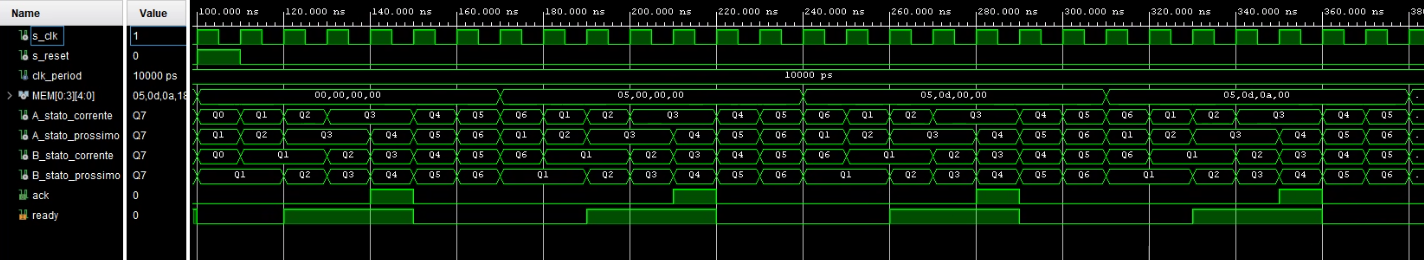
\includegraphics[width=16cm]{immagini/esercizio7/output_simulazione_7.1.png}
    \caption{Output della simulazione}
    \label{fig:notebook}
\end{figure}